\chapter{MC-SBD-STM Result}

In this chapter, we present the result from the \ac{MC-SBD} algorithm(the algorithm from now) on both the synthetic data and real experimental data on various materials. We first introduce a synthetic QPI-STM data generation process, build a corresponding metric system, and evaluate the performance of the algorithm on a wide range of synthetic data. Then we will show results in the real data, and evaluate it with a simple faithfulness metric. 

\section{MT-SBD-STM Result on synthetic data}
Evaluating the algorithm's performance on synthetic data is necessary, as in the real data we have less access to the ground truth of both kernel and activation. A good synthetic data set should thus capture the physical data generation process during an experiment. In this section, we showcase that the algorithm works well in a wide parameter spaces. We aim to achieve it by presenting an experiment-informed simulation method, build a metric system that evaluates the algorithm from 3 perspectives, and then present results that falls in different parameter spaces. Finally, we will discuss the cases where the algorithm failed and its potential reasons. 

\subsection{Synthetic Data Generation Process}
The synthetic data generation process follow closely with the convolutional model of QPI-STM that we established in Ch. 5. Mathematically, the synthetic data $Y(\omega)$ is generated via:
\begin{equation}
	Y(\omega) = \sum_i^s ( A_i(\omega) * X_i) + \beta. 
\end{equation} 

%A real STM grid map samples from a continuously varying Local density of states. However, due to the discrete nature of computer simulation, we need to make modifications and even compromises in designing the data generation process. 
\begin{figure}
	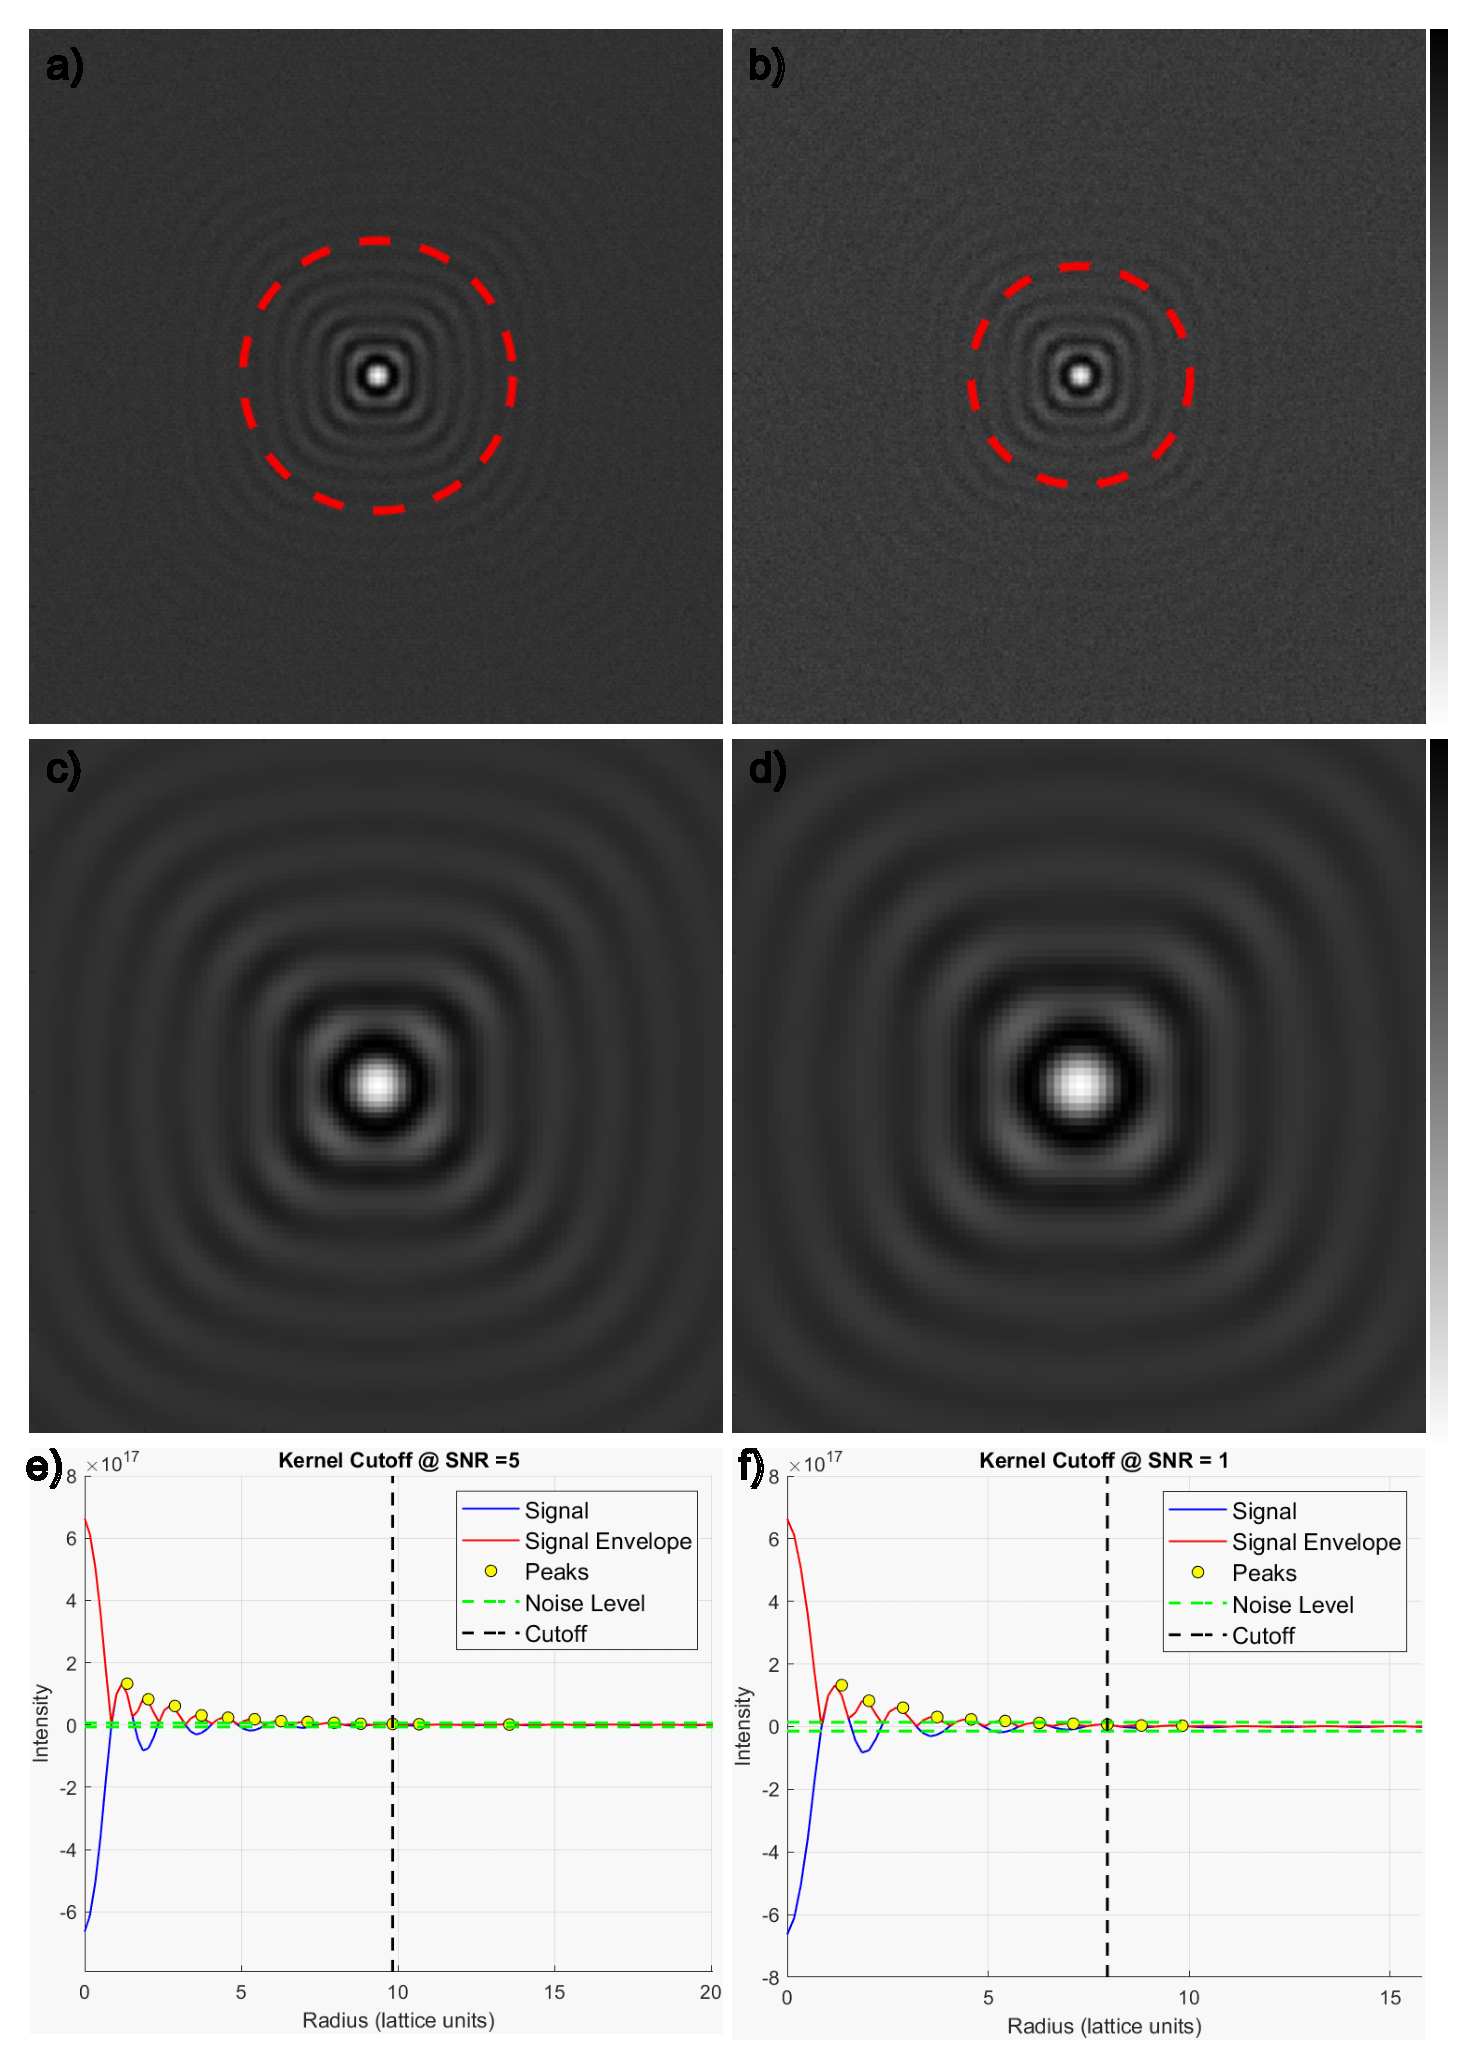
\includegraphics[width= \textwidth]{Ch7_kernel_size.pdf} 
	\centering
	\caption{}
	\label{fig:ch7_kernel_size}
\end{figure}

In practice, there are 4 parameters that dictates $Y(\omega)$, they are:
\begin{itemize}
	\item Signal to Noise Ratio($SNR$): the variance ratio between the noiseless kernel and the noise. This influence $\beta$ and $A_i(\omega)$, we will elaborate the latter influence later. 
	\item Observation lattice size($N_{obs}$): total number of lattice sites per side within the grid map. This dictates the physical size of the grid map. 
	\item Linear observation resolution($p$): number of pixels per lattice site, this is enforced to be an integer due to the discrete nature of simulation. 
	\item defect density($\rho_i$): number of defect i per lattice site. Practically, it is equivalent to the probability of a lattice site to host defect i, a formulation according to the statistical framework of defect we established in Ch. 4.
\end{itemize}
\begin{figure}
	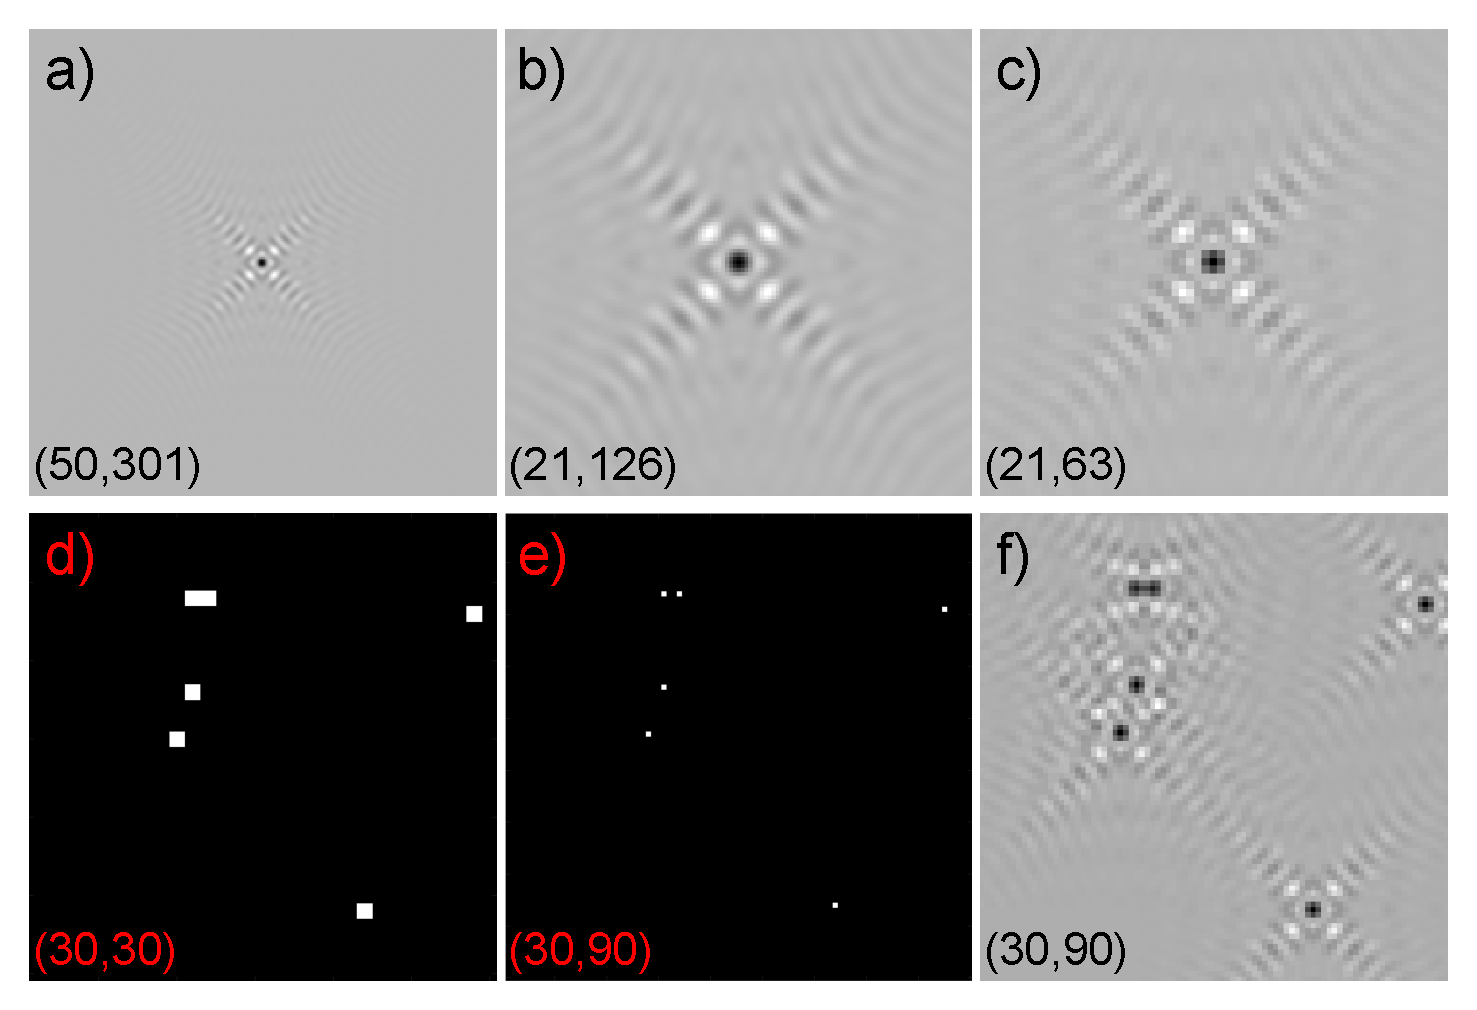
\includegraphics[width= \textwidth]{Ch7_synGen.pdf} 
	\centering
	\caption{}
	\label{fig:ch7syn}
\end{figure}

The step by step data generation process is illustrated in Fig. \ref{fig:ch7syn}. It is worth noting that we have a pair of numbers in the bottom-left corner of each subplot. Every pair indicates the observation lattice size and pixel size of this image. We first take the simulated \ac{LDOS} on the tight-binding model we built in Ch.4 and pick an energy slice, we generate a) with large $N_{obs}$ and dense pixels. Then we choose an an SNR-ratio $SNR$ and apply it onto a), due to the decaying nature of the \ac{QPI} pattern, we can draw an cutoff location where the signals are buried in the noise, as illustrated in Fig. \ref{fig:ch7_kernel_size}. This process gives us b), a truncated version of a) with noise added. a) and b) mimics the underlying \ac{LDOS} on the surface of the sample that \ac{STM} samples from. In real experiment, this sampling process turns the initially continuous \ac{LDOS} to a discrete grid map. Here, we model this processing through down sampling an initially dense grid($p=6$) b) with a smaller linear observation resolution $p=3$ and get c), our ground truth kernel $A^{gt}_i$; note that the down sampling only changes the pixel size, but keeps the spatial lattice size unchanged. The activation map is first generated in the lattice grid, as the impurities mostly sit on the lattice sites. Then we resize the activation map to match the linear resolution of the kernel and get e), our ground truth activation map $X^{gt}_i$. Finally, we use apply 2D linear convolution to $A^{gt}$ and $X^{gt}$ to get the ground truth observation for kernel $i$: $Y^{gt}_i$. We then repeat this process and composite different observations to construct the final observation $Y^{gt}= \sum_iY^{gt}_i$. 

Our simulation approach improves on two key limitations of the original method. First, in the original synthetic data generation workflow proposed by Cheung et al., the kernel was generated by simply selecting a target size and applying imresize to a large single-defect QPI simulation. This process arbitrarily rescales the entire QPI pattern without considering how far the signal meaningfully extends, leading to unphysical distortion of spatial features. In contrast, our method determines the kernel size based on where the QPI signal becomes indistinguishable from noise, with a defined SNR threshold. This ensures the kernel reflects the true spatial extent of the physically meaningful signal. Second, Cheung et al. placed impurities on a binary pixel grid without regard to the underlying lattice, allowing the impurities to appear off-site—a simplification that breaks down in most materials where defects are confined to lattice points. Our method instead defines the activation map on the actual lattice grid and ensures defects are positioned only at valid lattice sites. These two improvements—grounding the kernel in real signal decay and enforcing lattice-consistent activation—make our simulated data more faithful to experimental conditions and more reliable for algorithm benchmarking.

We now show some examples of the synthetic data generated to give some taste to the readers about how we tune the knobs and model datasets in different regimes. As illustrated in Fig. \ref{fig:synexample}, we first plot a reference observation $Y_a$ in a), with 2 different types of defects, $SNR = 5$, $N_{obs}=50$, linear resolution $p = 3$, density of individual type $\rho_i = 0.2 \%$. We can tune the density of individual defect type by changing $\rho_i$, an example is given in b), with $\rho_i$ doubled and other parameters unchanged. We can also tune the spatial resolution of the scan, by changing the linear resolution $p$, in c), we present a case where $p$ is doubled, modeling a case where we have grid map that is more fine-grained. Lastly, we can change the expand the physical coverage of the scan by modifying $N_{obs}$. Here, we doubled the $N_{obs}$ and plot the $Y_d$ in d). With these parameters, we can create a parameter space that covers a wide range of different datasets and then test the robustness of our algorithm. Before we do that, we first need to build a metric system that measures the goodness of reconstruction between the algorithm output and the ground truth data. 

\begin{figure}
	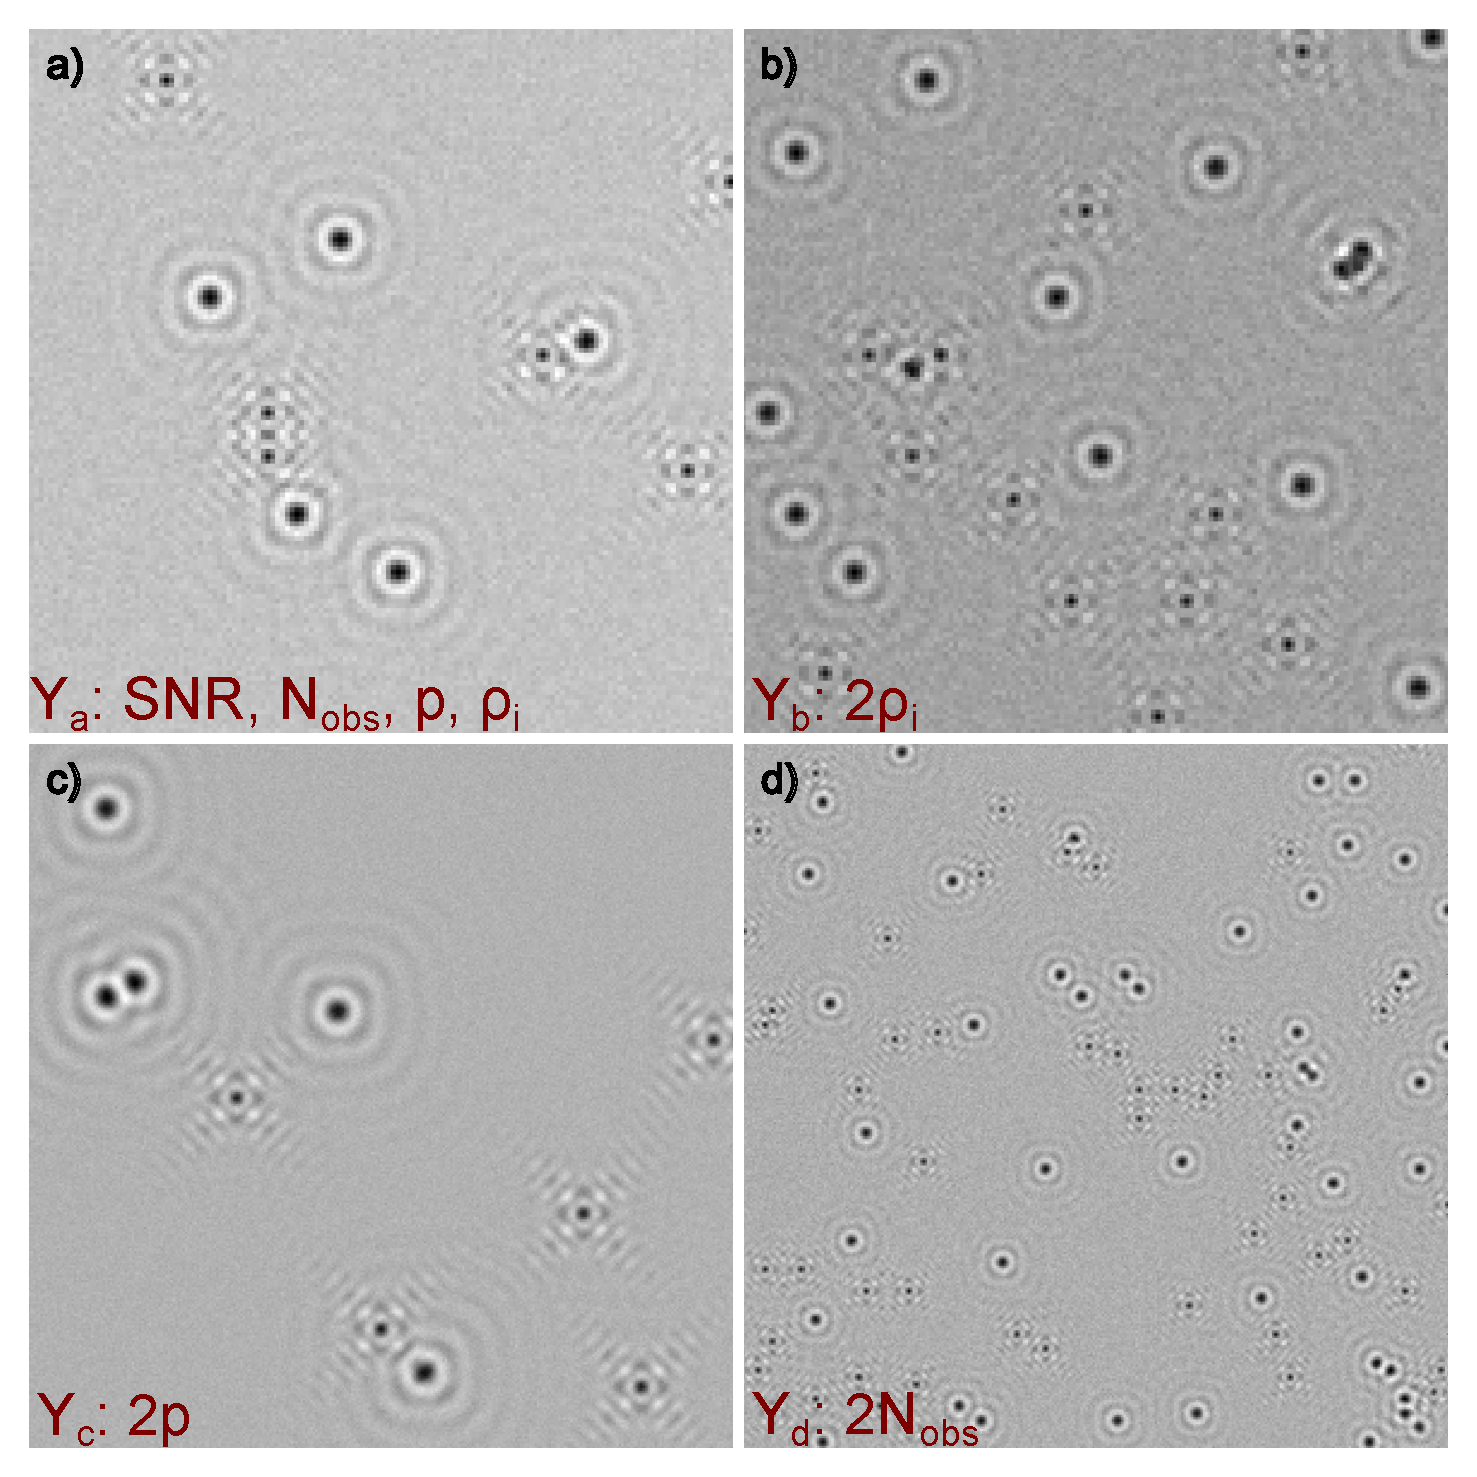
\includegraphics[width= \textwidth]{synGenExamples.pdf} 
	\centering
	\caption{}
	\label{fig:synexample}
\end{figure}

\section{MT-SBD-STM Metric system}
The MT-SBD metric system consists of four metrics. They are \textbf{Kernel Similarity(\textit{KS})}, \textbf{Activation Similarity(\textit{AS})}, \textbf{Observation fidelity(\textit{OF})}, and \textbf{Demixing score(\textit{DS})}. \textbf{\textit{KS}} and \textbf{\textit{AS}} requires the ground truth data, which can only be accessed in synthetic data, the rest of metrics can be applied to both synthetic data and real data. We will illustrate these 4 metrics through an example run of the algorithm on a synthetic observation. 

We illustrate the data generation process, the algorithm initialization and result in Fig. \ref{fig:metric}. Given $SNR = 5$, $N_{obs}=50$, linear resolution $p = 3$, density of individual type $\rho_i = 0.3\%$, we generate a synthetic observation: 
\begin{equation}
	\label{eq:observation}
	Y = \sum_i A^0_i * X^0_i + noise.
\end{equation} The observation is plotted in e), with kernels and their activation maps shown in a) to d). We then feed $Y$ and the randomly initialized kernels $A_i^{init}$ into the \ac{MC-SBD} algorithm and get results shown in h) to l). 

\begin{figure}
	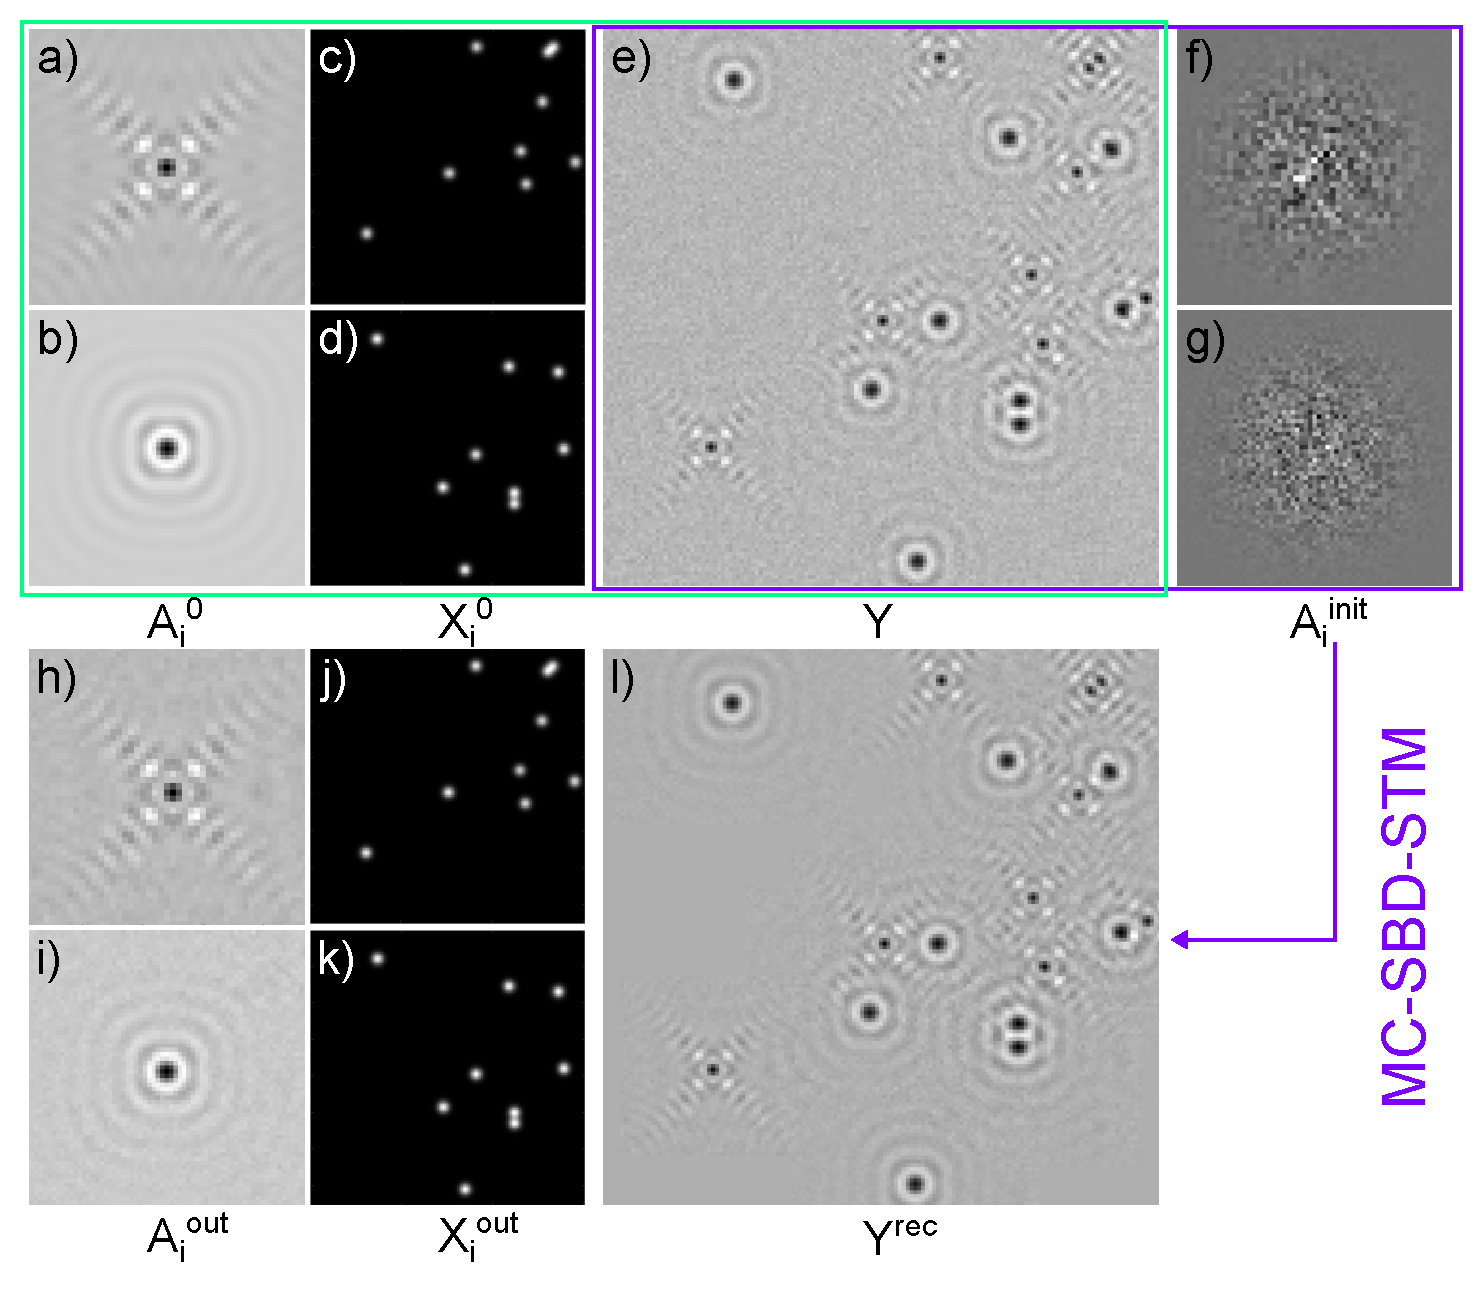
\includegraphics[width= \textwidth]{metric1.pdf} 
	\centering
	\caption{Example run of \ac{MC-SBD} algorithm on a synthetic dataset.}
	\label{fig:metric}
\end{figure}

The algorithm outputs $A_i^{out}$ and $X_i^{out}$. It successfully demixed two types of kernels and reconstructed an observation $Y^{rec}$ that is similar to the original observation $Y$. Note that $Y^{rec} = \sum_i A^{out}_i * X^{out}_i$, not a direct output from the algorithm. Moreover, all the activation maps shown in Fig. \ref{fig:metric} are generated by applying a Gaussian window to the original discrete activation. Detailed reasons will be given when elaborating the Activation Similarity metric. 

Before showing the resulting metric scores for this example run, we first elaborate how each metric is established and what aspects of performance does it evaluate. 
\begin{itemize}
	\item \textbf{Kernel Similarity(\textit{KS})}: 
	\begin{equation}
		\textbf{\textit{KS}} = \frac{\operatorname{FT}(A_i^0)_{\textit{flatten}} \cdot  \operatorname{FT}(A_i^{out})_{\textit{flatten}}}{\vert \vert \operatorname{FT}(A_i^0)_{\textit{flatten}} \vert \vert \cdot  \vert \vert \operatorname{FT}(A_i^{out})_{\textit{flatten}}\vert \vert}
	\end{equation}
	\textbf{\textit{KS}} directly evaluate how well the outcome kernel matches with the ground truth kernel, by calculating the cosine similarity between the ground truth kernels and the output kernels in the q-space. Performing Fourier transform first enforces centering of the \ac{QPI} pattern, thus the cosine similarity is only sensitive to the actual feature of the kernel, but robust against any in-plane shift in real-space kernel. 
	
	\item \textbf{Activation Similarity(\textit{AS})}: 
	\begin{equation}
		\textbf{\textit{AS}} = \frac{\operatorname{GW}(X_i^0)_{\textit{flatten}} \cdot  \operatorname{GW}(X_i^{out})_{\textit{flatten}}}{\vert \vert \operatorname{GW}(X_i^0)_{\textit{flatten}} \vert \vert \cdot  \vert \vert \operatorname{GW}(X_i^{out})_{\textit{flatten}}\vert \vert}
	\end{equation}
	\textbf{\textit{AS}} evaluate how well the outcome activation map matches with the ground truth activation map, by calculating the cosine similarity between the Gaussian windowed ground truth activation and the Gaussian windowed output activation. The GW is applied to reduce the influence of tiny misalignment while preserving the dominating features of the activation map. This allows us to construct a more continuous and robust metric to evaluate the performance. More specifically, the square GW is defined as: $g(r)= e^{\frac{r^2}{2 \sigma}}$, where $\sigma = \operatorname{min}(\frac{1}{3}\sqrt{\frac{-ln(0.95)}{\rho \pi}}, \frac{\textbf{\textit{kernel size}}}{10})$. $\rho$ is the fraction of active pixels in the activation map, and \textbf{\textit{kernel size}} is the side length of the kernel associated with this activation. This means if activations are sparse (low density), the filter becomes broader to average over a wider area, while if activations are dense, the filter stays sharper.
	
	\item \textbf{Observation fidelity(\textit{OF})}
	\begin{equation}
		\textbf{\textit{OF}} = \operatorname{variance}(noise)/\operatorname{variance}(Y_{residual}),
	\end{equation}
	where $Y_{residual} = Y - Y_{reconstructed} = Y - \sum_i(A^{out}_i * X^{out}_i)$, and $noise$ is the noise term in Equation. \ref{eq:observation}. In an ideal case, where $A^{out}_i = A^{0}_i$ and $X^{out}_i = X^{0}_i$, the discrepancy between $Y_{reconstructed}$ and $Y$ will be at the noise level. Thus, a successful run of the \ac{MC-SBD} algorithm will give \textbf{\textit{OF}} $\approx$ 1. We can further exemplify this by plotting all observations and noise level under the same color limit as shown in Figure. \ref{fig:OF}, we can see that c) and d) have similar variance. Note that the observation fidelity is the ultimate metric we will use to evaluate the performance of the reconstruction in real data. 
	
	\item \textbf{Demixing Score(\textit{DS})}:
	\begin{align}
		\textbf{\textit{DS}} &= 1 - \operatorname{softIoU}(X_i^{out},X_j^{out}) \\
		&= 1 - \frac{\sum(\operatorname{min}((X_i^{out})_{flatten}, (X_j^{out})_{flatten}))}{\sum(\operatorname{max}((X_i^{out})_{flatten}, (X_j^{out})_{flatten}))}
	\end{align}
	\textbf{\textit{DS}} evaluates how little two activation maps of different kernel types overlap using soften Intersection over Union(softIoU). The rational is that the probability of two different types of defects sitting on the same lattice site is near zero; Thus, a successful demixing should give \textbf{\textit{DS}} close to 1. Note that this metric relies solely on the output activation and thus can also be applied to real data.  
\end{itemize}

The scores of the four metrics for this example run are listed in Table \ref{table:metric}, all of which indicate a successful execution of the algorithm. In particular, we observe a perfect match for the activation maps, as illustrated in Figure \ref{fig:metric} (panels c, d, j, k). Regarding kernel similarities, both \textbf{\textit{KS}} values exceed 0.95, indicating a near-perfect match. To examine this more closely, Figure \ref{fig:KS} presents the detailed \ac{QPI} patterns in both real and reciprocal spaces for type two. From left to right, the three columns show the noiseless ground truth kernel, the output kernel, and the noisy ground truth kernel.

Since the input observation $Y$ is noisy, it would be natural to expect the output kernel to resemble the noisy ground truth kernel. However, the output kernel actually captures more structural information than the noisy ground truth, as evident in the reciprocal \ac{QPI} patterns. For example, panel e shows faint square arcs outside the high-intensity diamond features, which also faintly appear in panel d but are entirely absent in panel f. This is a surprising, yet consistent, outcome across multiple datasets.

The reason is that while the noise is random, the \ac{MC-SBD} algorithm identifies repetitive units (the kernels) throughout the entire observation, and the signals from all activation sites are taken into account. As a result, the reconstructed kernel is effectively an average over all the instances. It is thus denoised and resembles the noiseless ground truth more closely than the noisy input. This highlights the advantages of this novel approach compared to conventional methods like simple cropping.

Nevertheless, despite this denoising effect, the output kernel still retains some random fluctuations, which makes a perfect match with the noiseless ground truth impossible. In fact, these random fluctuations are exploited by the algorithm to further reduce the residual, contributing to the overfitting factor of $\textbf{\textit{OF}} = 1.34 > 1 $, This elevated \textbf{\textit{OF}} suggests mild overfitting, likely driven by those same random fluctuations in the reconstructed kernel. A detailed comparison between $Y^{res}$ and $Noise$ is provided in Figure. \ref{fig:OF}
% todo: can make a plot of all averaged vs out kernel.  

\begin{table}[h]
	\label{table:metric}
	\centering
	\begin{tabular}{|l|c|c|}
		\hline
		\textbf{Metric} & \textbf{Kernel 1} & \textbf{Kernel 2} \\
		\hline
		Kernel Similarity & 0.9749 & 0.9701 \\
		\hline
		Activation Similarity & 0.9983 & 0.9994 \\
		\hline
		Separation Score & \multicolumn{2}{c|}{0.9999} \\
		\hline
		Observation Fidelity & \multicolumn{2}{c|}{1.34} \\
		\hline
	\end{tabular}
	\caption{Quantitative evaluation of kernel and activation similarity, separation, and observation fidelity for two kernel types.}
\end{table}

\begin{figure}
	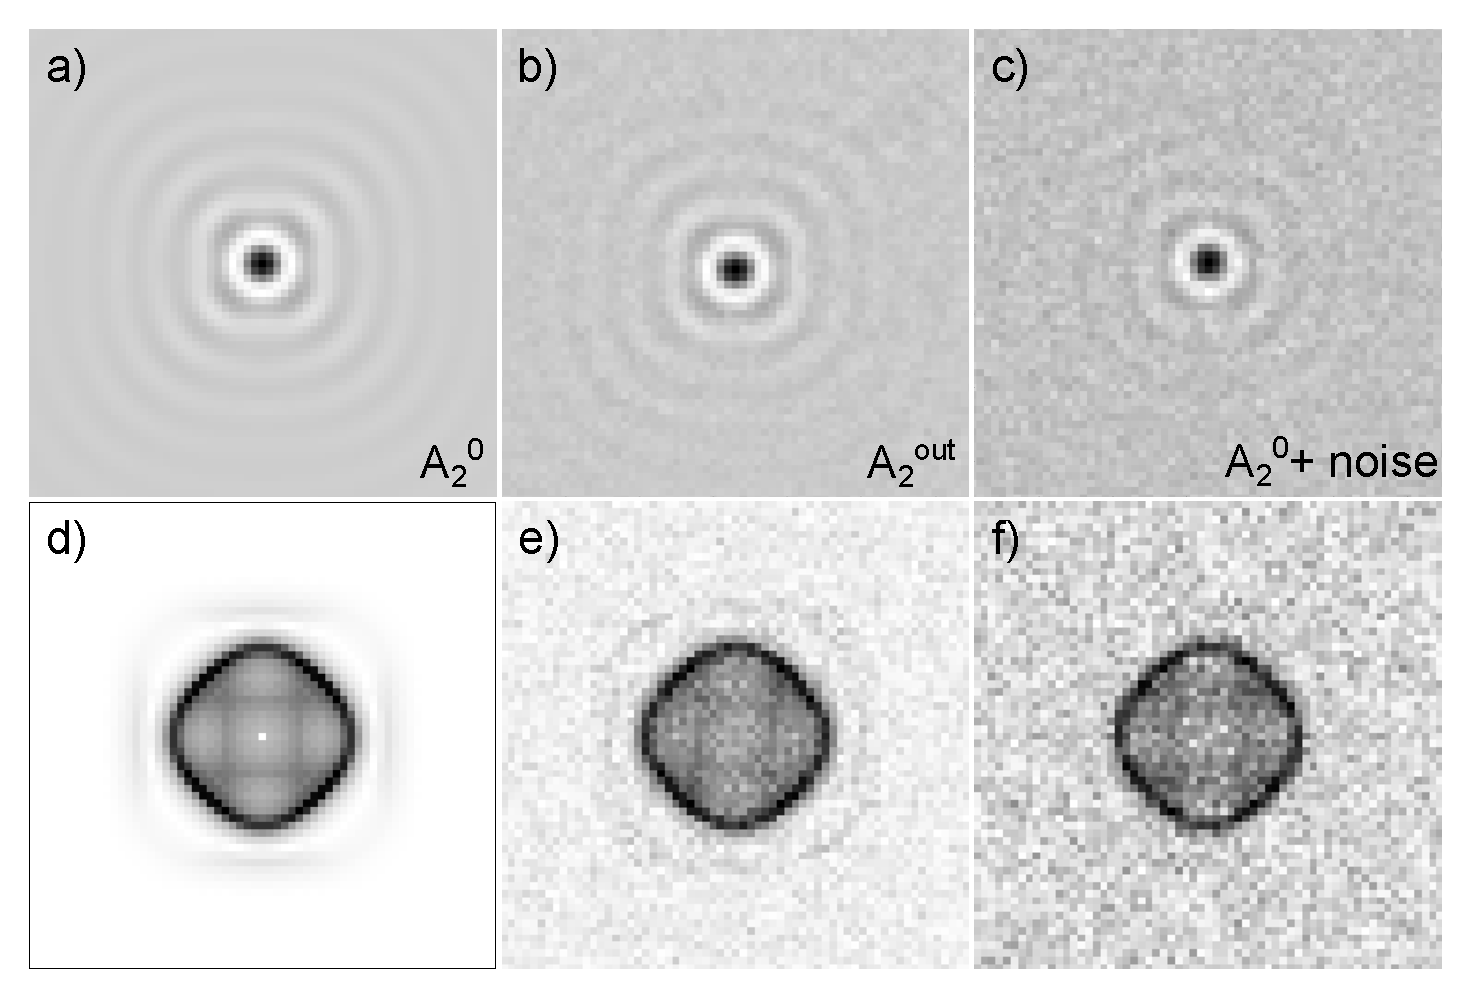
\includegraphics[width= \textwidth]{KS.pdf} 
	\centering
	\caption{Kernel comparison in both real and reciprocal space}
	\label{fig:KS}
\end{figure}

\begin{figure}
	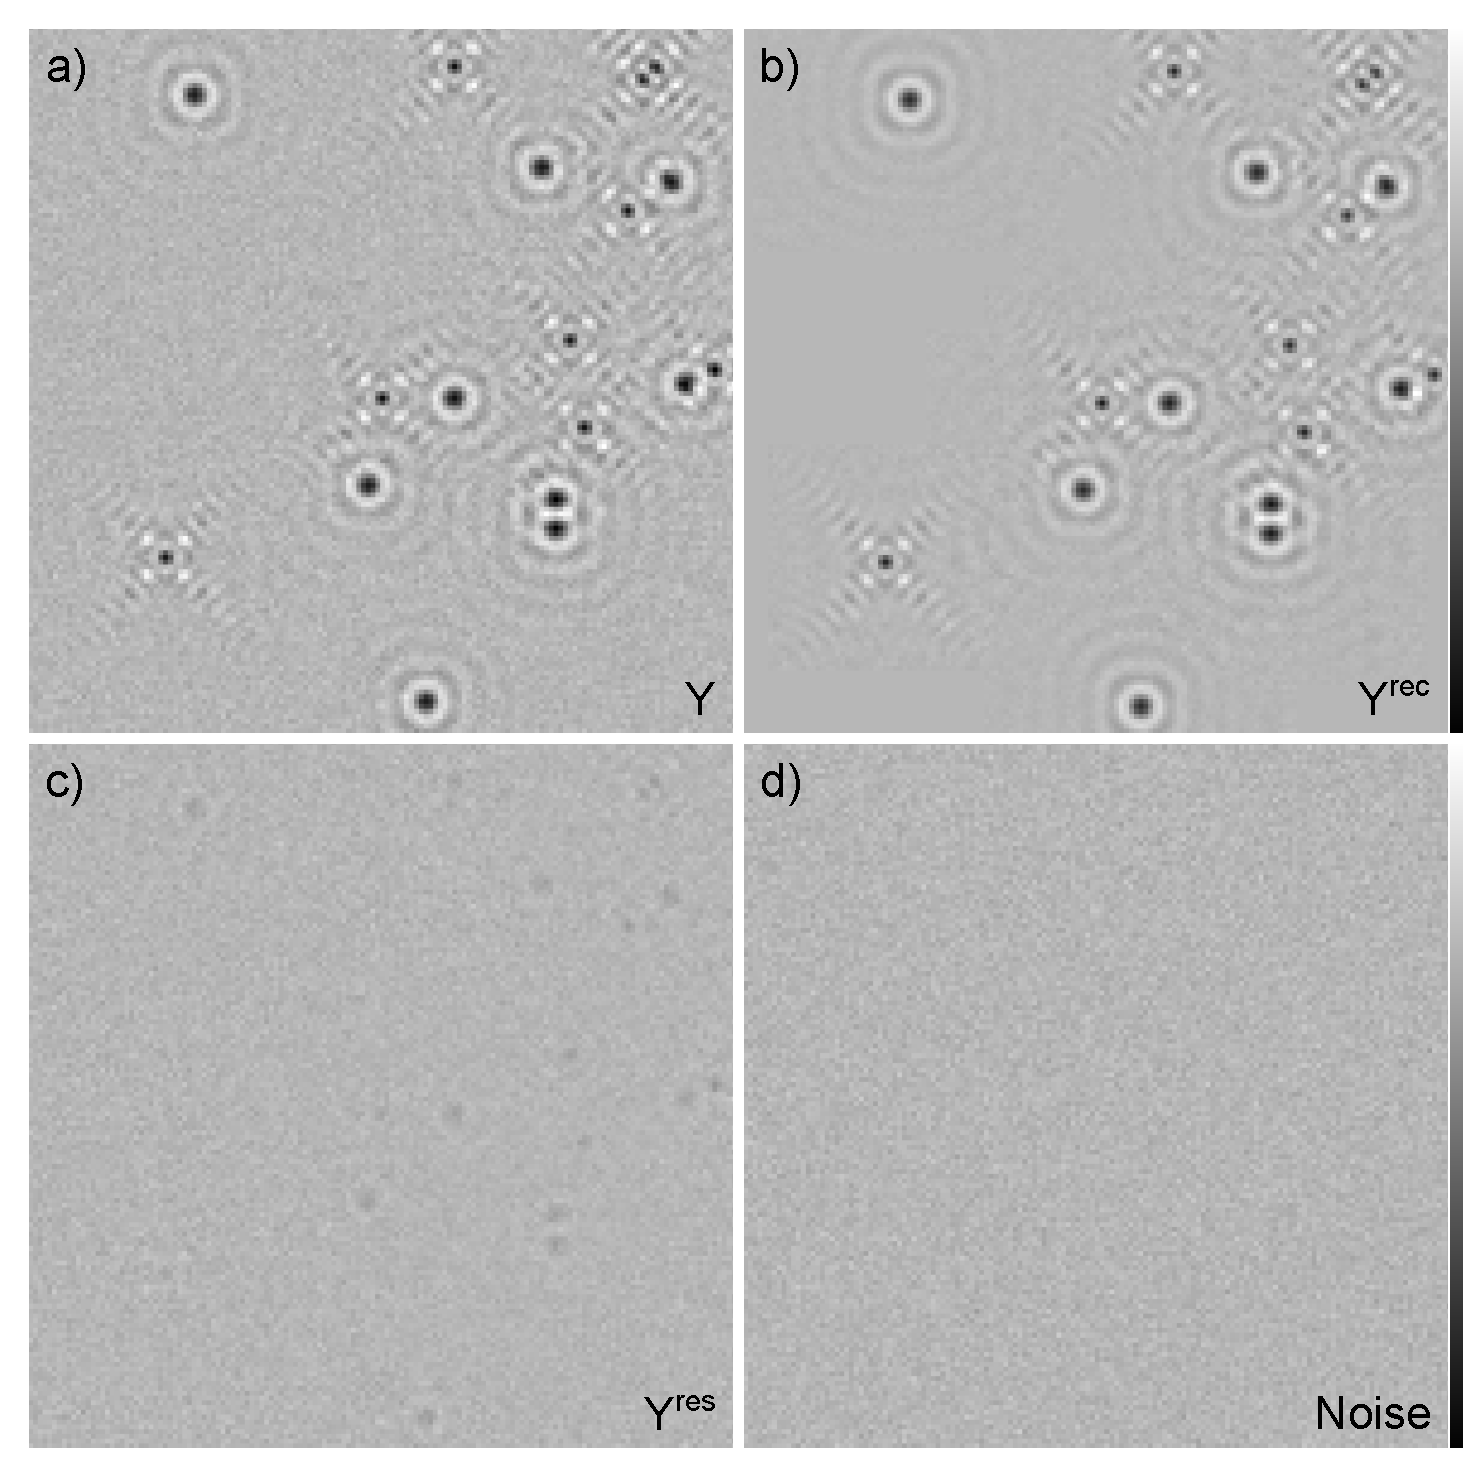
\includegraphics[width= \textwidth]{OF.pdf} 
	\centering
	\caption{Illustration of the observation fidelity(OF)}
	\label{fig:OF}
\end{figure}


\section{Benchmark tests on the dataset parameter space}
Now that we understand what the algorithm can achieve and how to evaluate its performance, it is time to address under what conditions it performs well. Analogous to evaluating an output $y$ given $f(x)=y$, where one must consider both the system parameter space defining the function $f$ and the input parameter space determining $x$, we must consider two aspects of our problem. First, the \ac{MC-SBD} algorithm itself involves several free parameters, such as the number of decomposition iterations, the sparsity regularizer $\lambda$, and the faint factor $\beta$. We have explored this system parameter space and identified sets of optimal values, the details of which will be provided in the supplementary material.

This section focuses on the second aspect: the dataset parameter space, which governs the input observations. This analysis addresses how broad the input landscape can be while still yielding reliable algorithmic performance, and, in the context of experimental data, what types of measurements are most likely to produce successful outcomes. This in turn provides potential guidelines for experimental data acquisition, ensuring the disentanglement of different \ac{QPI} contributions from various defects.

To this end, we generate physics-informed synthetic data with varying parameters and test our algorithm across a range of dataset regimes. Recall that we can explore datasets in these 4 axis: 
\begin{itemize}
	\item 1. noise level - $SNR$, 
	\item 2. Range of the grid map - $N_{obs}$, 
	\item 3. defect density for each type - $\rho_i$,
	\item 4. Spatial resolution of the grid map - $p$.
\end{itemize}
Since it is a common practice to set the spatial resolution as either 2 or 3 when taking a grid map, we will not explore this axis and set $p=3$ for all our datasets. 

Apart from the above parameters, we also tuned the number of different types of defects(or kernel types). However, due to the drastic increase in computational expense with increasing kernel types, we first run a full exploration of the parameter spaces with 2 types of kernels, and then followed by toy runs with kernel types = 3 and 4. 

In the full exploration runs we ran on 2 types of kernels, we run the algorithm on 3 trials with different datasets. The datasets with different parameter sets are listed in Table.\ref{table: parameter_space}. In total, 180 different observations are generated to cover defect density from sparse to dense, grid map of sizes range from $10^2$ to $10^4$ nanometer squares(given a normal bond length is around 2-5 angstrom), and signal to noise ratio from as low as 0.5 to 3. We then collect the results from all the trails and plot the corresponding metrics to a 3D phase space plot as shown in Figure. \ref{fig:phase_space}. There are two things to evaluate, the kernel and activation maps, since they can behave differently within the parameter space, we make one subplots each. On the left we use \textbf{\textit{KS}} to evaluate the performance on the kernel recovery, and on the right, since there are two metrics defined to evaluate the activation maps, for convenience, we use \textbf{combined score(\textit{CS})}:  
\begin{equation}
	\textbf{\textit{CS}} = \sqrt{\textbf{\textit{AS}} \cdot \textbf{\textit{DS}}}.
\end{equation} 

Each marker on the 3D plot represents a single dataset generated in our experiments. As shown in Table~\ref{table:parameter_space}, some datasets share the same initialization parameters; however, because the activation maps are generated randomly, these datasets are not identical. For parameter combinations that occur more than once, the metric value displayed at that point is the average of the metrics from all corresponding datasets. In total, there are 132 non-overlapping datasets represented in the plot. A triangular marker indicates the case of overlapping datasets, and we take the average of the corresponding metrics, whereas a circular marker indicates a non-overlapping case. The color of each marker indicates the average value of metrics computed over both kernel types within each individual dataset. The metric colorbar of two subplots are defined in the same way; It has 3 sections, red section ranging from $[0.0, 0.85]$, yellow section from $[0.85,0.98]$, and the green section for metrics within $[0.98,1]$. The colorbar is designed around 2 thresholds that are empirically chosen based on manual judgments from STM researchers. $0.85$ is the pass line for a given recovery, below which the recovery is considered failed. Values above $0.98$ gives recoveries that are indistinguishable from the ground-truth kernels and activation maps, and thus is considered a success. It is also worth noting that the ground-truth kernels used in \textbf{\textit{KS}} calculations are noiseless ground-truth, like panel a) in Figure. \ref{fig:KS}. This sets a even higher standard for the algorithm. 

\subsection{discussion on the phase space}
In general, the algorithm works in most of the phase space we explore, more specifically, it is very successful on datasets with low to medium defect concentration, medium to big $N_{obs}$, and higher SNR. This give us a reference on the robustness of this algorithm, and a rough estimate on the algorithm's effectiveness on real data within these regimes.

We also observe that the two metrics we used respond differently with different parameters. Kernel similarity is more sensitive to the size of scans, with smaller scan sizes, for example when $N_{obs} = 50$, the kernel reconstruction works less well. 

This is likely because of the denoising effect that we discussed; At fixed defect density, the number of occurrence of each kernel drops as we decrease $N_{obs}$, this weakens the denoising effect and makes the output kernels more noisy and less similar to the noiseless ground truth kernels.  
Comparing at Figure. \ref{fig:metric} panel a) and b),  

The activation combined score is more sensitive to the defect density, with large defect densities. 
\begin{table}[h!]
	\label{table: parameter_space}
	\centering
	\begin{tabular}{|l|c|c|c|}
		\hline
		\textbf{Trial} & \textbf{Defect Density} & \textbf{N\_obs} & \textbf{SNR} \\
		\hline
		1 & $[1.0e{-3},\ 1.8e{-3},\ 3.2e{-3},\ 5.6e{-3},\ 1.0e{-2}]$ & $[50,\ 100,\ 150,\ 200]$ & $[1,\ 3,\ 5]$ \\
		2 & $[1.0e{-3},\ 2.4e{-3},\ 5.6e{-3},\ 1.3e{-2},\ 3.2e{-2}]$ & $[50,\ 100,\ 150,\ 200]$ & $[1,\ 2,\ 3]$ \\
		3 & $[1.0e{-3},\ 3.2e{-3},\ 1.0e{-2},\ 3.2e{-2},\ 1.0e{-1}]$ & $[50,\ 100,\ 150,\ 200]$ & $[0.5,\ 1,\ 3]$ \\
		\hline
	\end{tabular}
	\caption{Parameter spaces for the 3 runs. In total 180 datasets where generated to explore 3 axes of parameters.}
\end{table}

\begin{figure}
	\centering
	\makebox[\textwidth][c]{%
		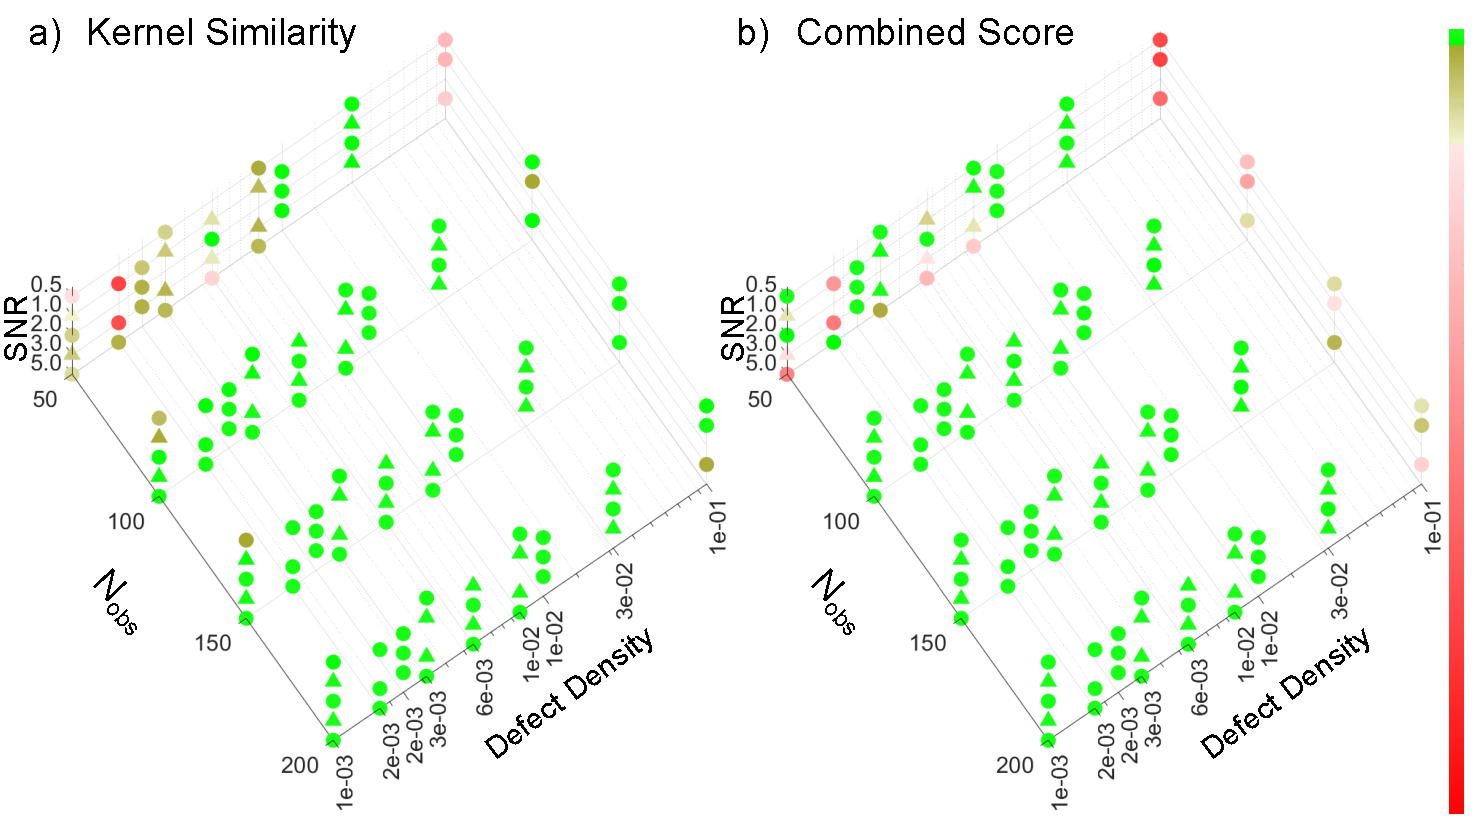
\includegraphics[width=1.5\textwidth]{total_metric_space.pdf}
	}
	\caption{Metrics phase space}
	\label{fig:phase_space}
\end{figure}

\begin{figure}
	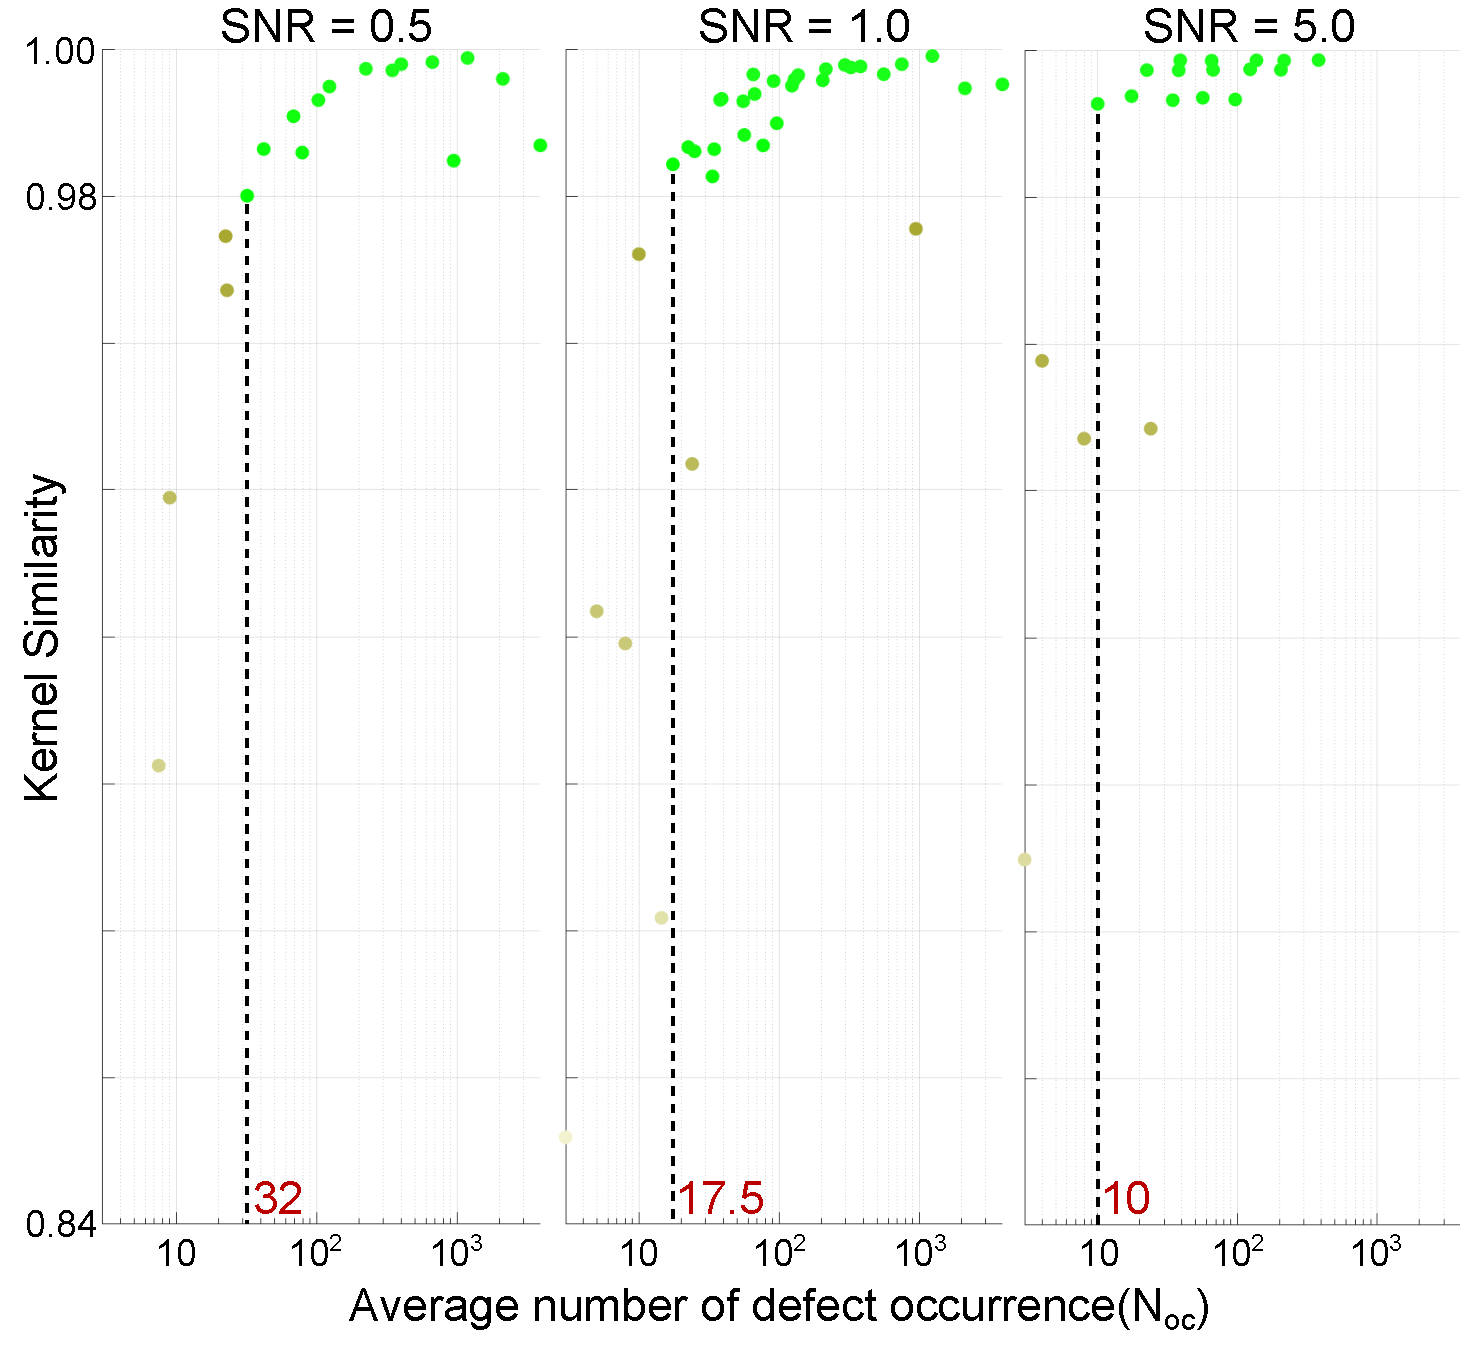
\includegraphics[width= \textwidth]{KS_vs_N.pdf} 
	\centering
	\caption{}
	\label{}
\end{figure}


\section{MC-SBD-STM on real data}
This section aims to demonstrate the application of \ac{MC-SBD} algorithm to real experimental data. We first elaborate the layers of complexity posed by real experimental data compared to the synthetic data. We then address the additional complexity by introducing a preprocessing pipeline that removes some common experimental artifacts and standardizes the experimental data condition before we apply the algorithm. At last, we apply the whole workflow to several experimental datasets and discuss the results. 

\subsection{real data complexity}
The phase space analysis in the last section showed the algorithm can worth robustly in vast regime of synthetic datasets. However, despite the effort we made to generate experiment-informed synthetic data, the real data might deviate from the synthetic data due to the occurrence of experimental artifacts. We thus need to discuss these additional layers of complexity and seek a way to remove them. 

%What define a success in real data? It really depends on the questions we try to answer. But we can roughly define a ladder of the success. Given a 3D grid map with spatial and energy dimensions: $x*y*V$, the lowest level of success is, we can run the algorithm 
%The lowest level of success is, given a 2D energy slice of the grid map, we can reconstruct The highest level of success is that, given a 3D grid map with spatial and energy dimensions: $x*y*V$, we 
\subsection{preprocessing pipelines}
\subsection{Ag}
\subsection{ZrSiTe}
\subsection{PtSn4}
\subsection{Potential use in other materials}

\section{Conclusion}
\ac{MC-SBD} algorithm grant us the impurity-dependent resolution of STM-QPI data, and helps us answer:
\begin{itemize}
	\item 1. At a given energy, is there any special states associated with different impurities?
	\item 2. What are the energy dispersion features of these impurity-dependent states?
\end{itemize} 
\subsection{regime it works and doesn't}
\subsection{Recipe to take data for MC-SBD}
\subsection{Future directions}